%\documentclass{article}
%\usepackage{graphicx,subfigure}
%\usepackage{caption,rotating}
%\begin{document}

\begin{figure}[!h]
\centering
\captionsetup{width=0.92\textwidth}
 \subfigure[Sheep w479 Wrinkled]{
%    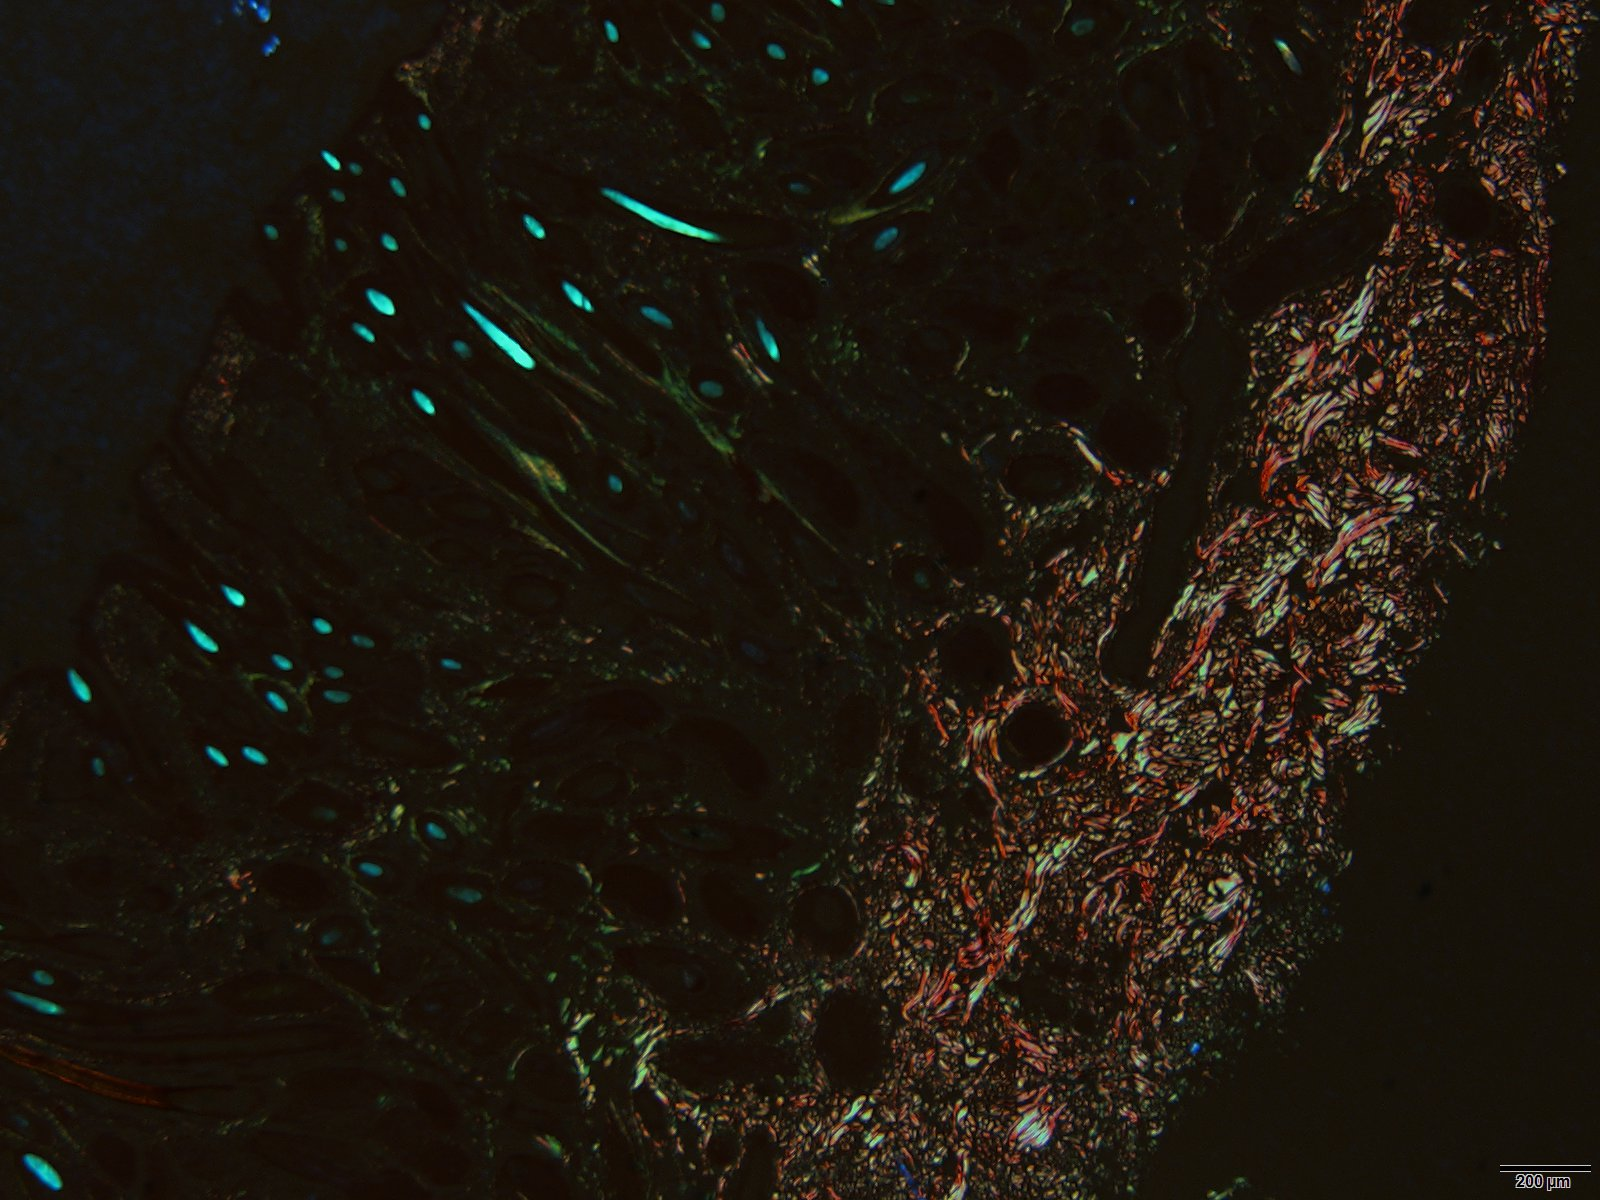
\includegraphics[scale=0.20]{w479-2_rigid_PSR_stain_polarised.jpg}
%   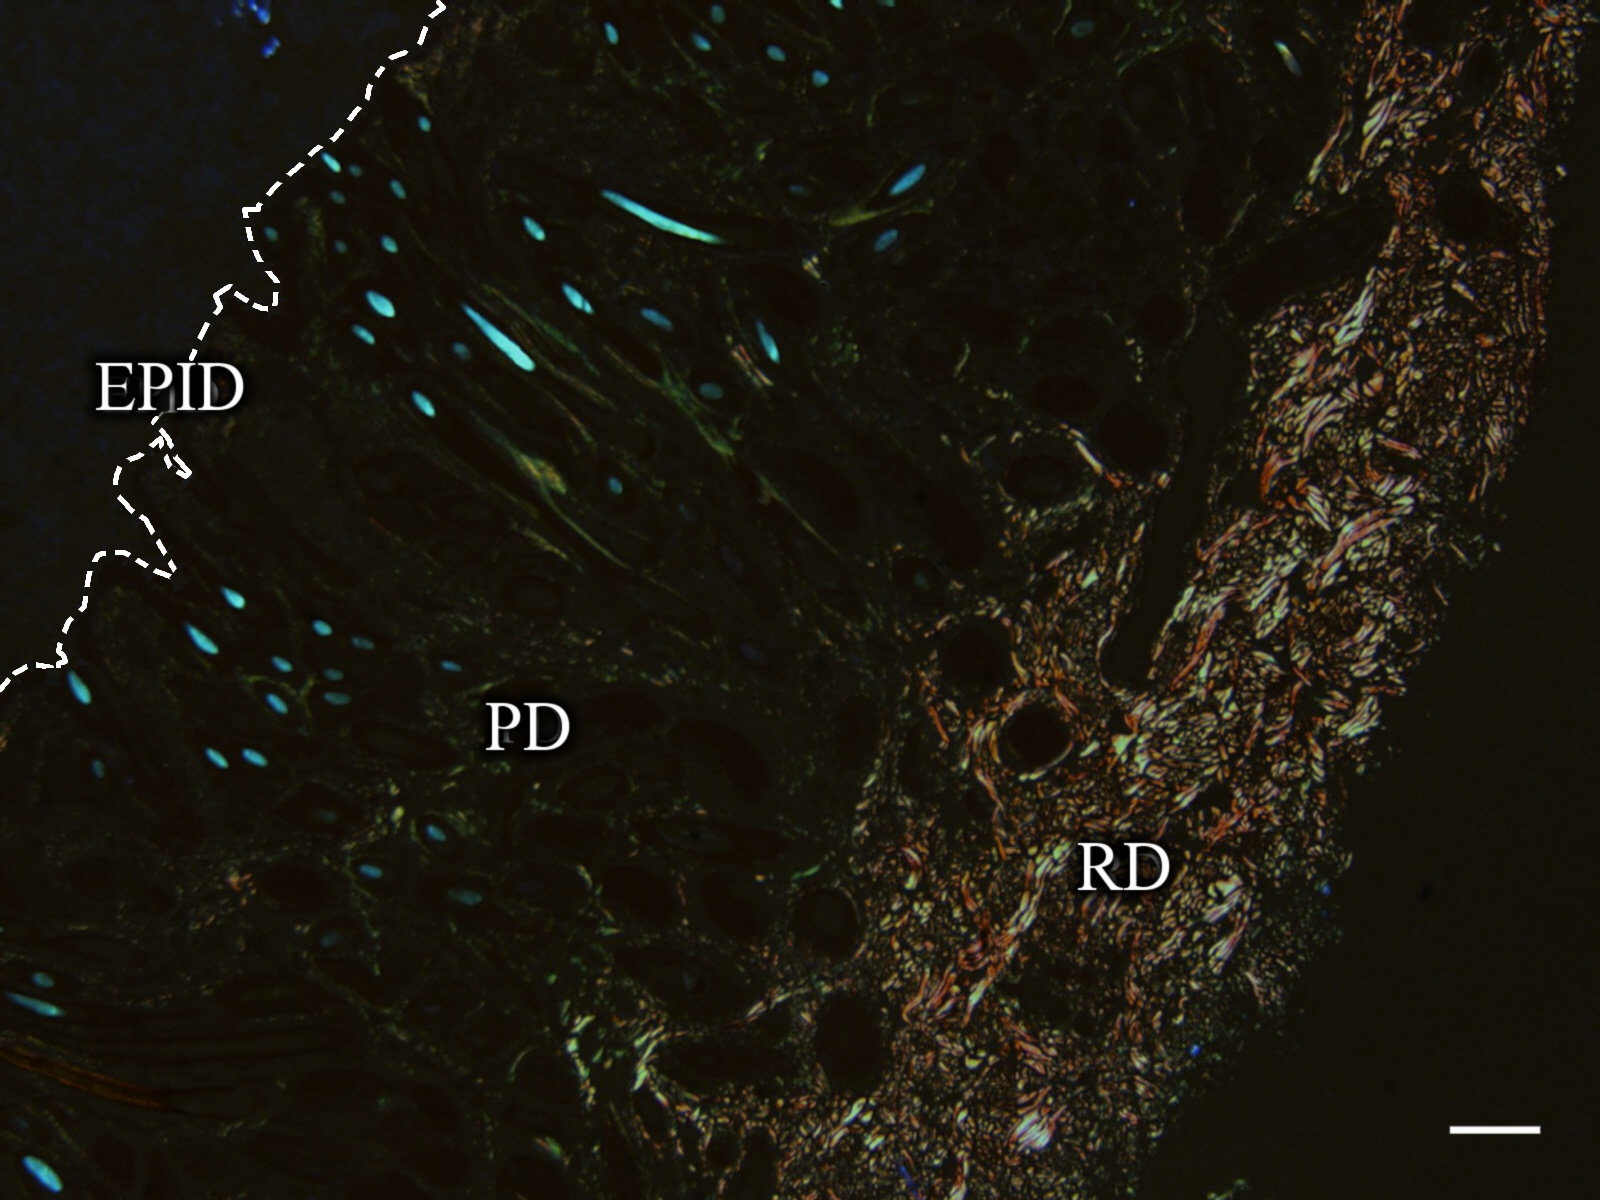
\includegraphics[scale=0.10]{fig9a.jpg}
    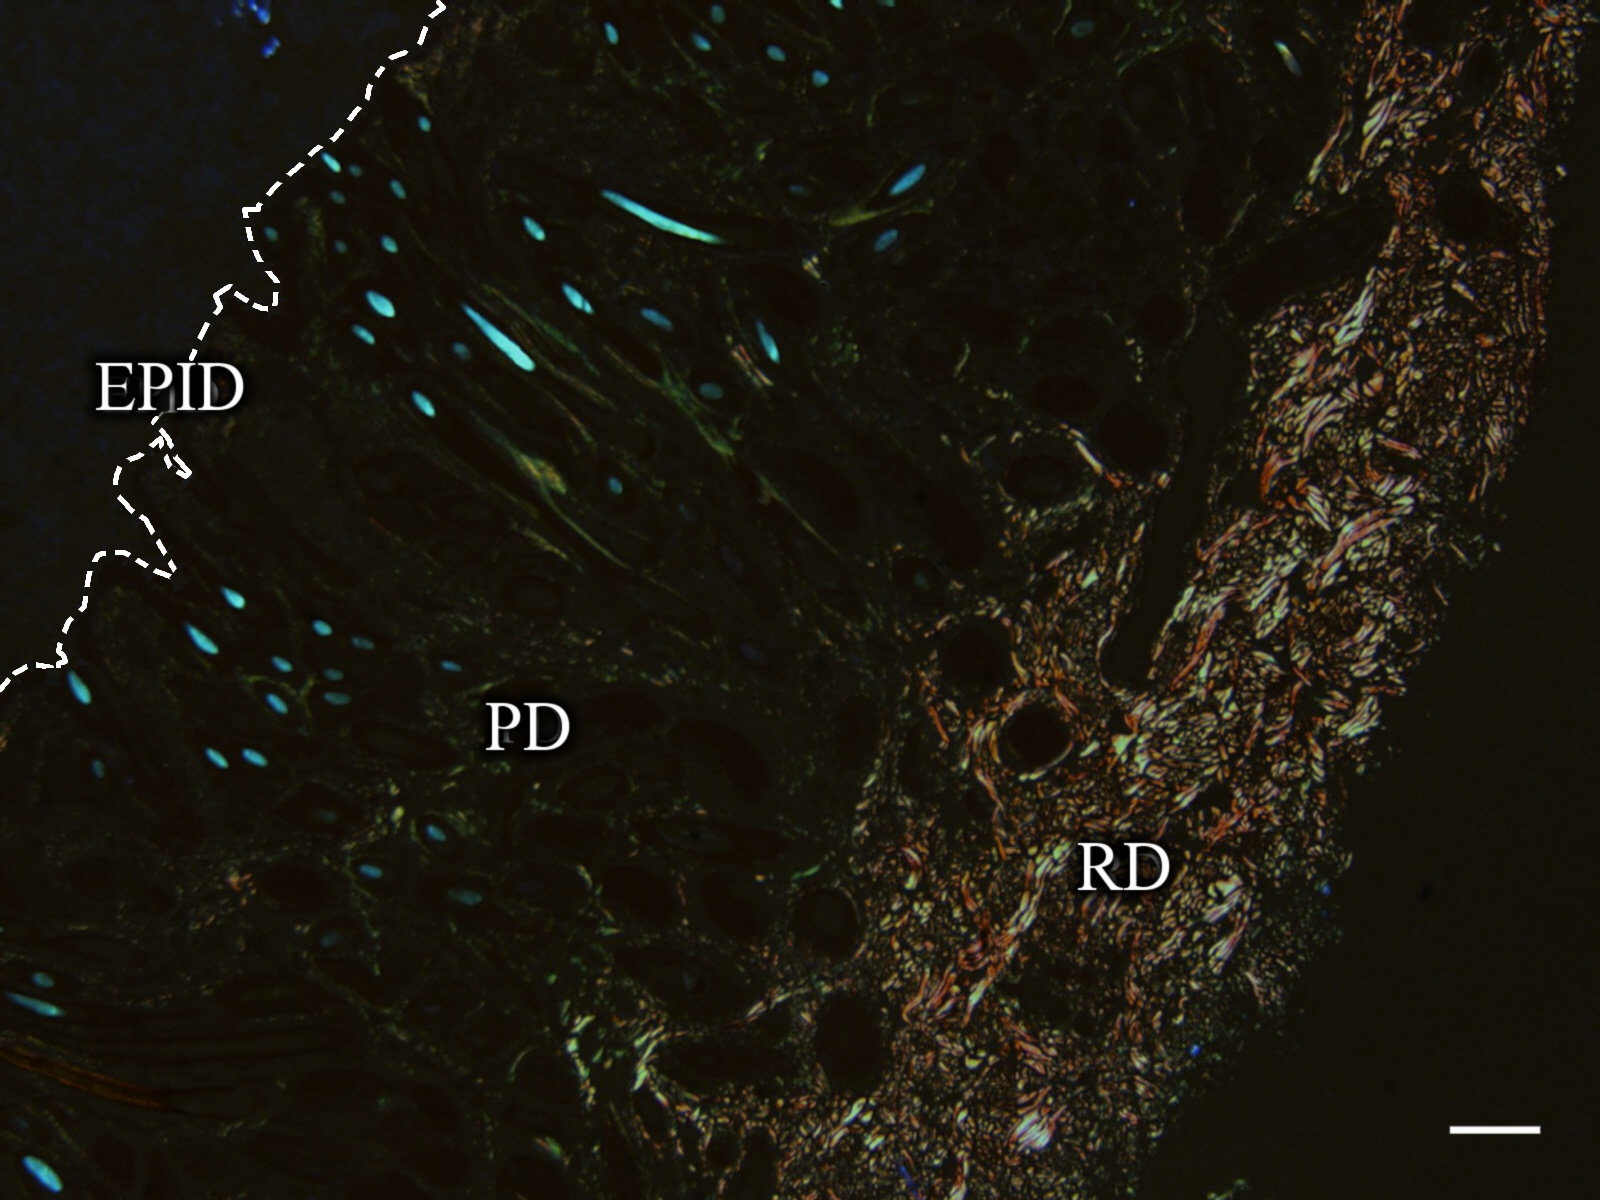
\includegraphics[width=0.45\textwidth]{fig9a.jpg}
% 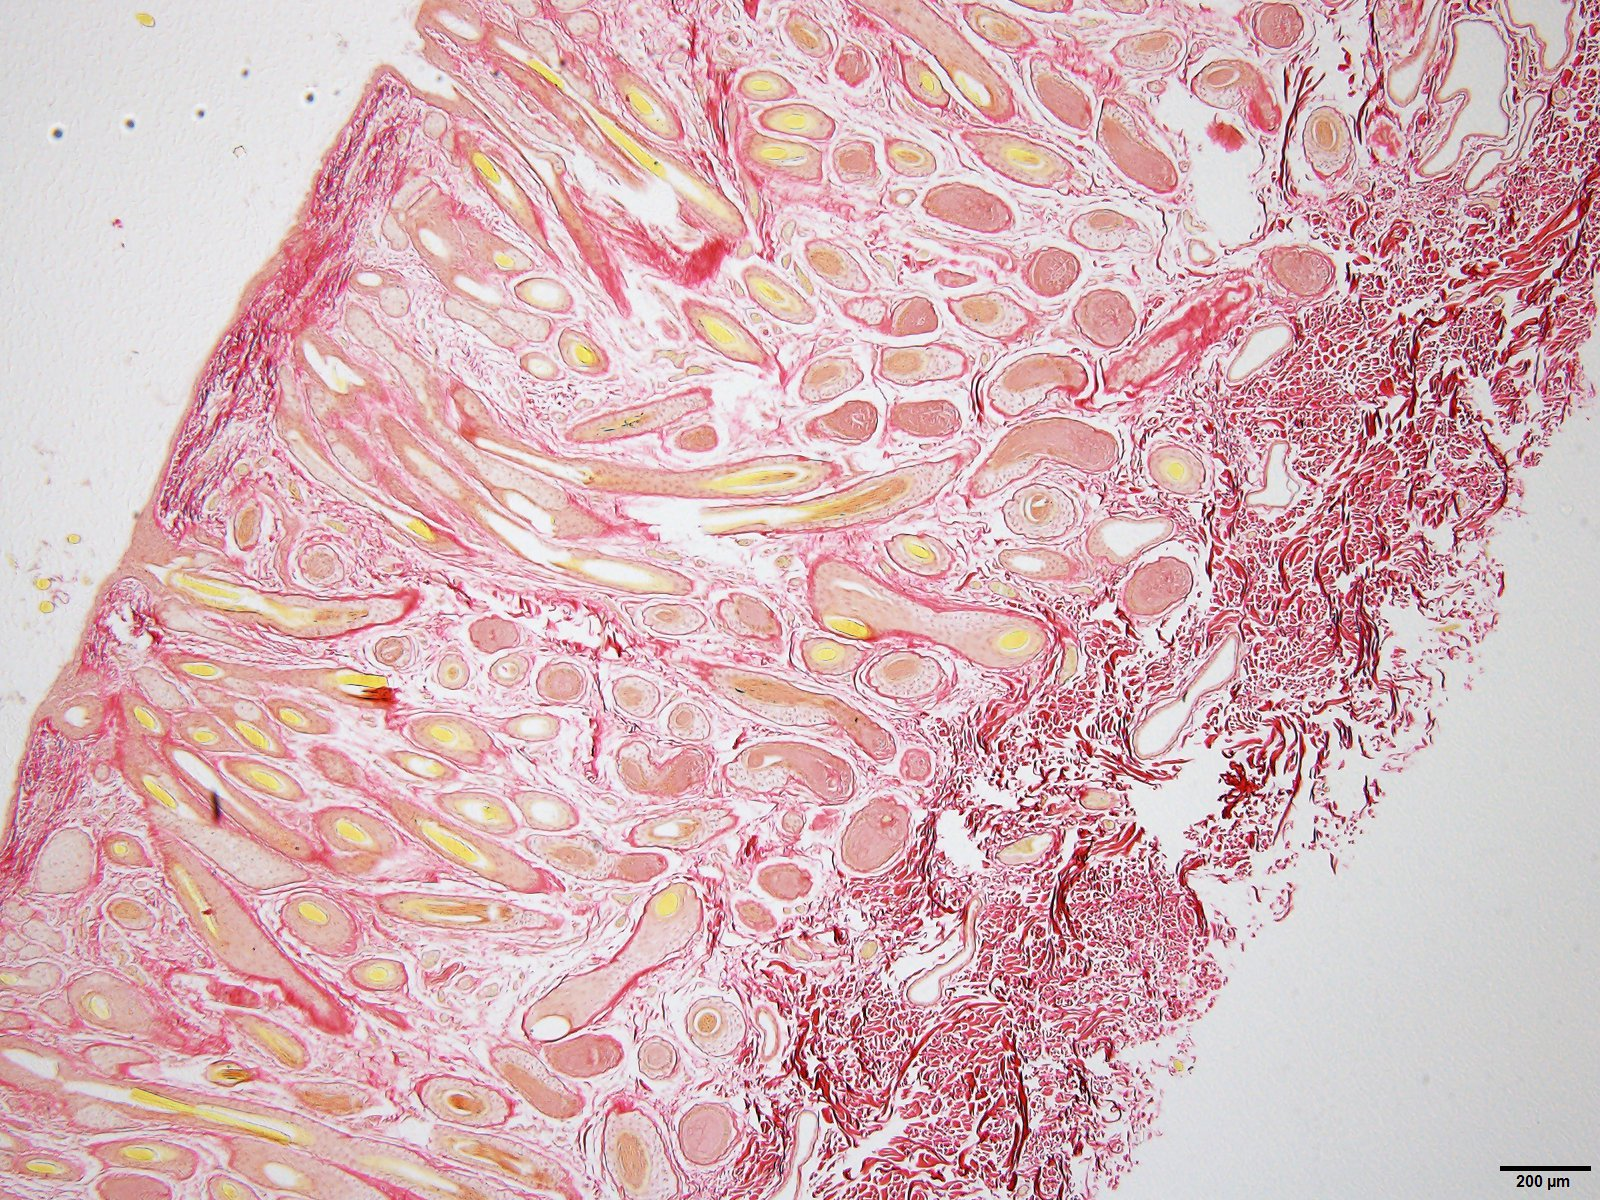
\includegraphics[width=1.0\textwidth]{w479-2-rigid.jpg}
  }
 \subfigure[Sheep w490 Wrinkle-free]{
%    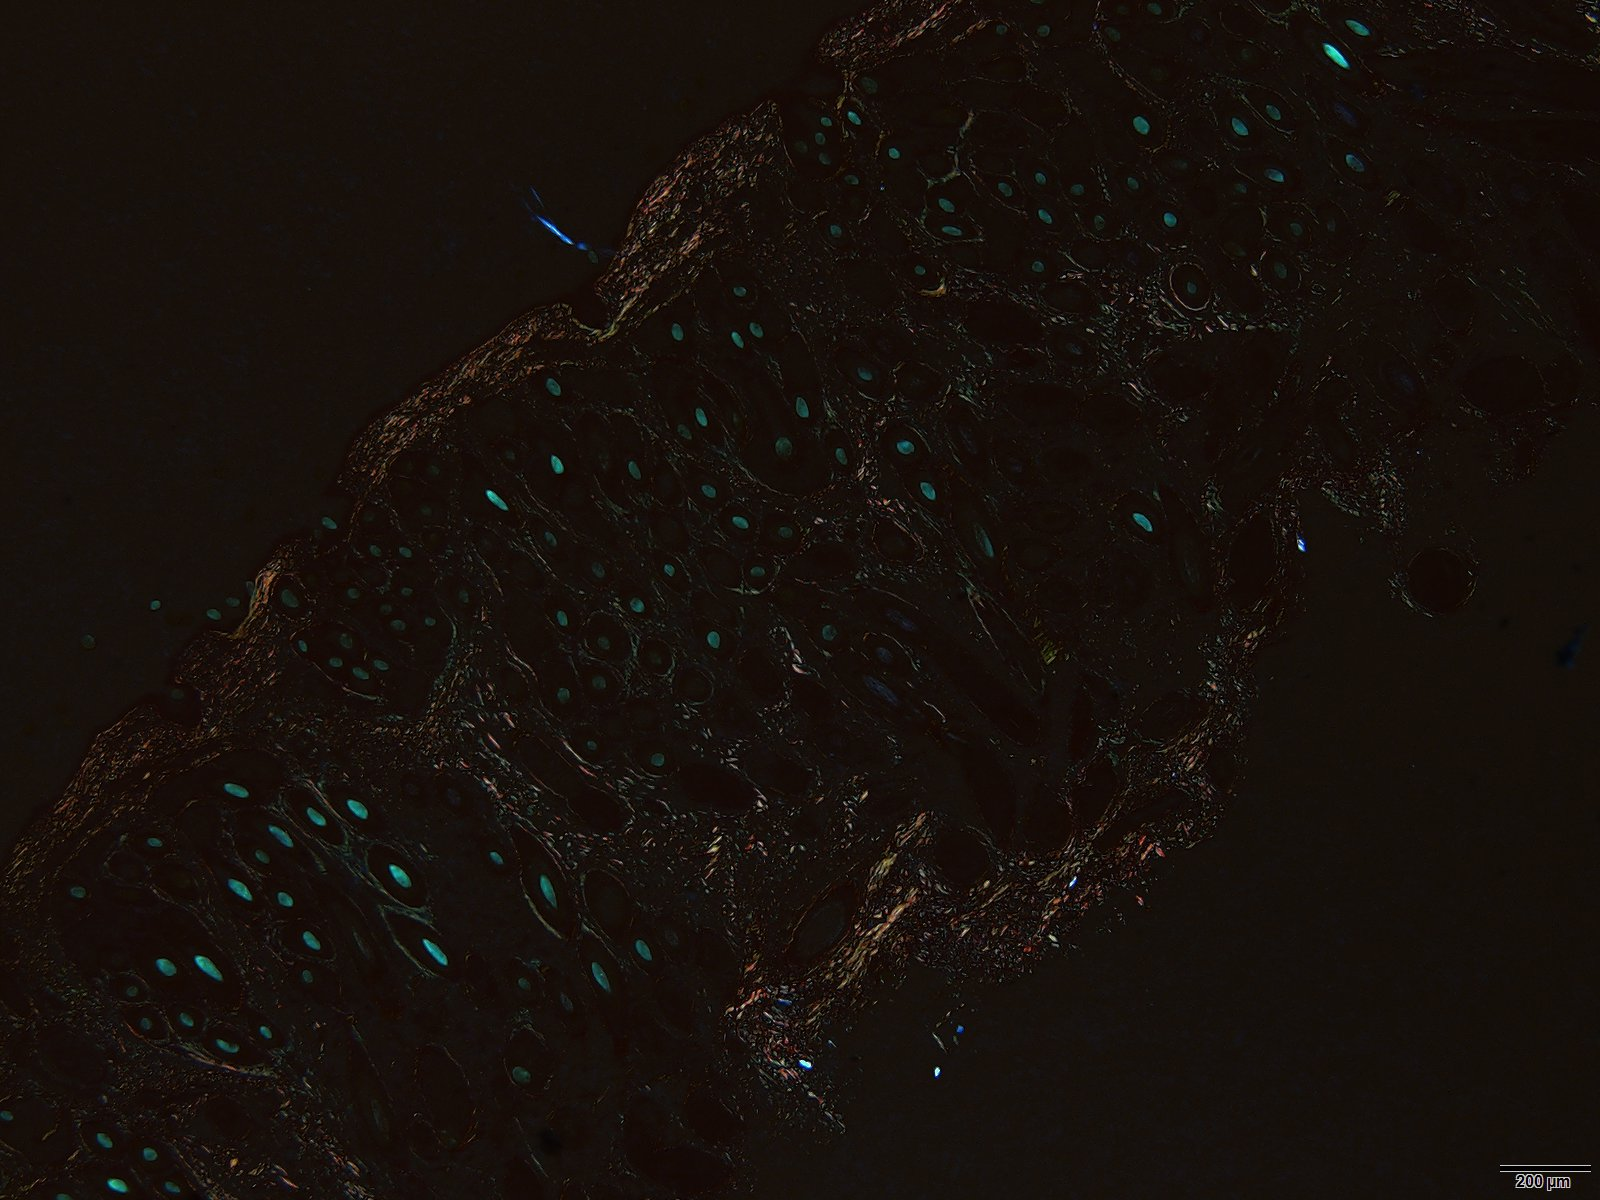
\includegraphics[scale=0.20]{w490-2_supple_PSR_stain_polarised.jpg}
%   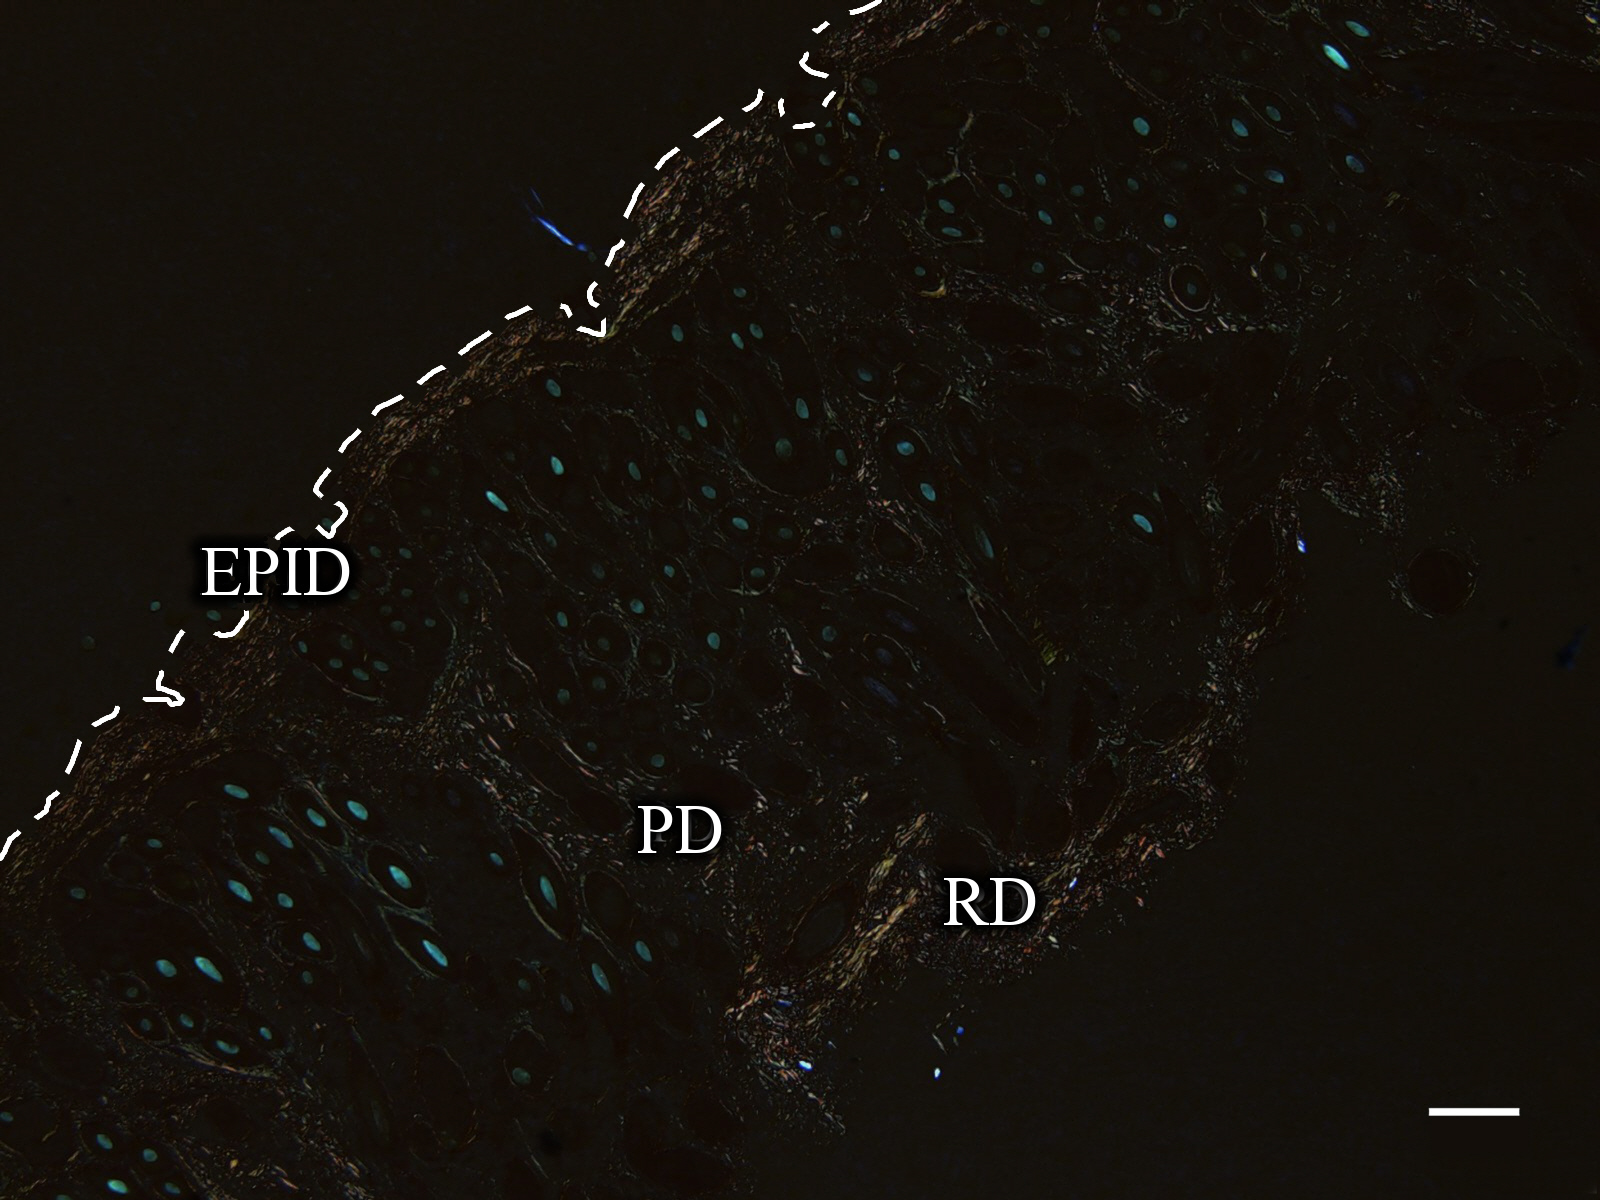
\includegraphics[scale=0.10]{fig9b.jpg}
    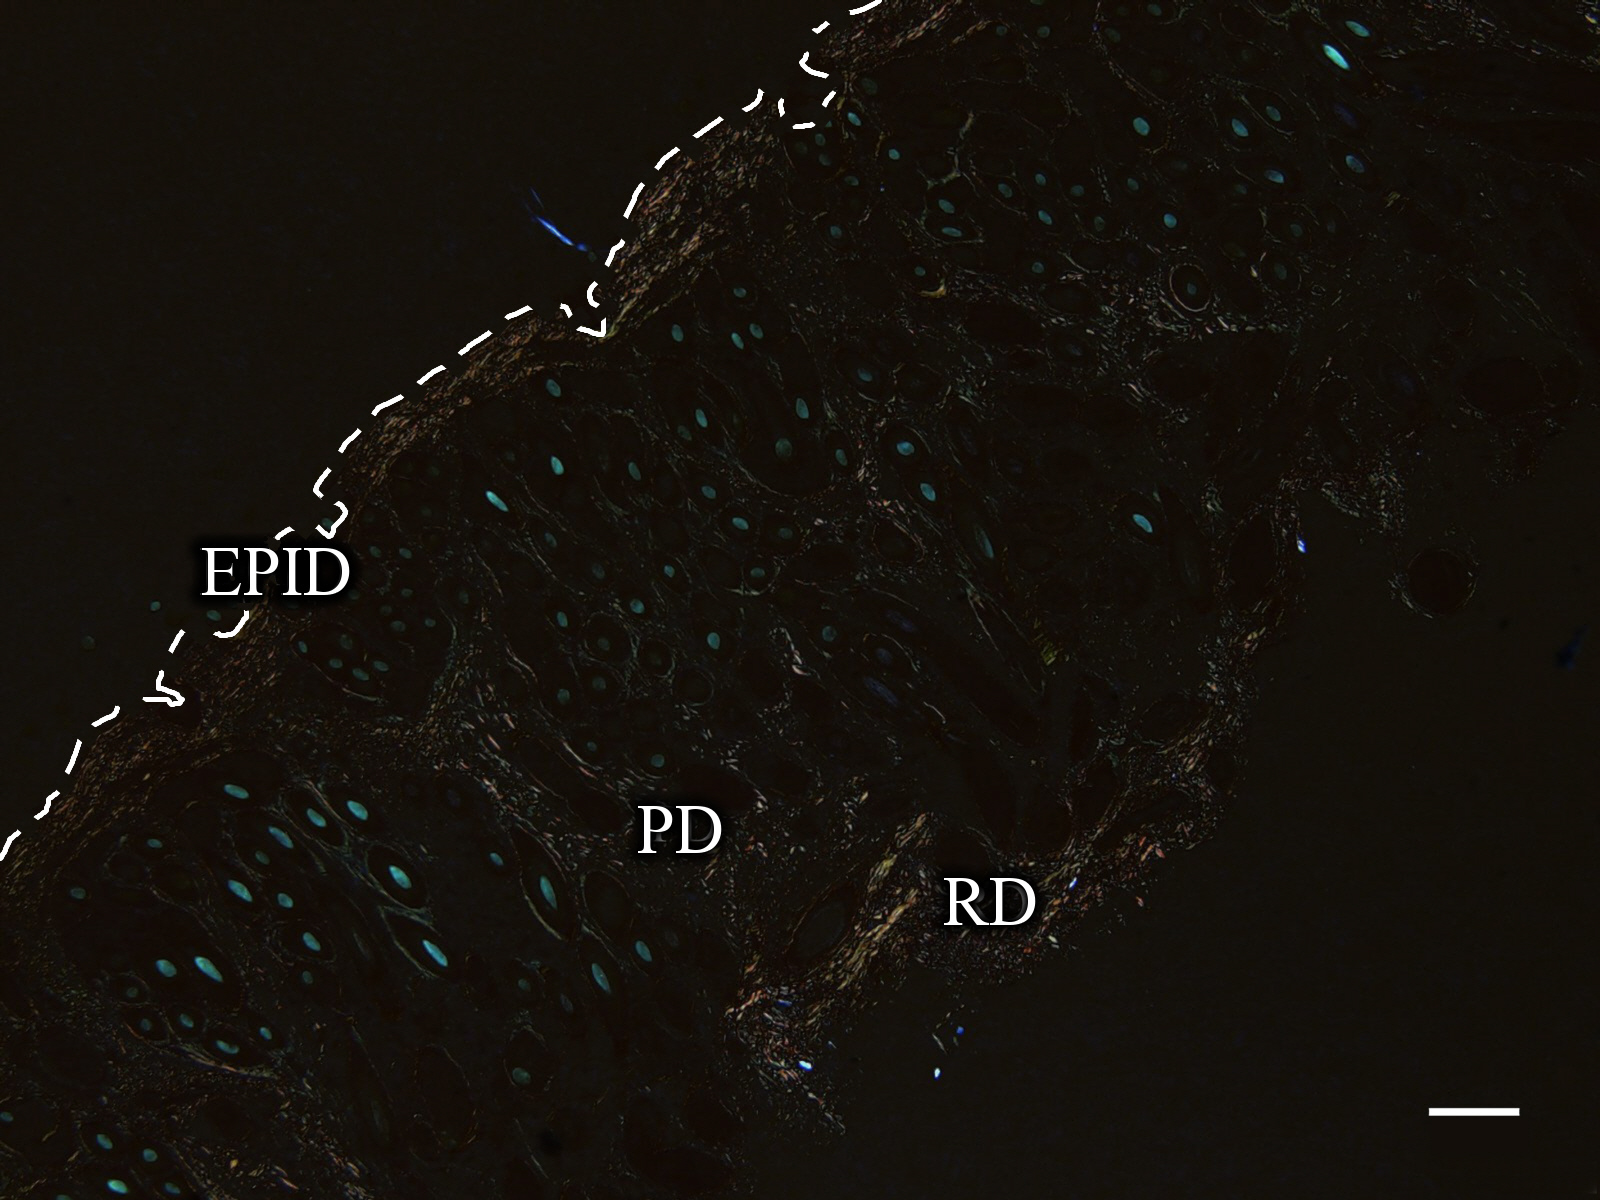
\includegraphics[width=0.45\textwidth]{fig9b.jpg}
  }
  \caption{Vertical sections from a wrinkled (a) and a wrinkle-free (b) sheep from Trial 1 flock 2 stained with PSR and examined with polarised light and a 4x objective. Skin layers are: {\bf EPID} epidermis, {\bf PD} papillary dermis, and {\bf RD} reticular dermis. Epidermal surface is marked with a dotted line. Scale bar is $200\mu m$. }
\vfill
  \label{fig:polar}
\end{figure}

%\end{document}

